\documentclass[10pt,conference]{IEEEtran}
%\IEEEoverridecommandlockouts
\usepackage[spanish,es-tabla]{babel}
\usepackage[spanish]{babel}
\renewcommand{\baselinestretch}{1.5}     %interlineado
\usepackage[utf8]{inputenc} 
\usepackage[square,numbers]{natbib}
\bibliographystyle{abbrvnat}
\usepackage{float}                      % para usar [H]
\usepackage{amsmath,amssymb,amsfonts}
\usepackage{graphicx}
\usepackage{textcomp}
\usepackage{xcolor}
\usepackage{ragged2e} % \justify

%---------- encabezado pagina
\usepackage{fancyhdr}
\pagestyle{fancy}
\fancyhf{}
\rhead{\thepage}
\renewcommand{\headrulewidth}{0pt}
%-----------------


%-----------------
\def\BibTeX{{\rm B\kern-.05em{\sc i\kern-.025em b}\kern-.08em
    T\kern-.1667em\lower.7ex\hbox{E}\kern-.125emX}}
%__________

\title{Algoritmos Metaheurísticos \\ {\Large Inteligencia Artificial 1}}
%--------------------------------------------
\author{
\IEEEauthorblockN{1\textsuperscript{do} Angely Mendez}
\IEEEauthorblockA{\textit{Escuela de Informática} \\
\textit{Universidad Nacional de Trujillo}\\
Trujillo, Perú \\
t052701020@unitru.edu.pe}
\and
\IEEEauthorblockN{2\textsuperscript{ero} Ciara Mendez}
\IEEEauthorblockA{\textit{Escuela de Informática} \\
\textit{Universidad Nacional de Trujillo}\\
Trujillo, Perú \\
t022700920@unitru.edu.pe}
}

%%--------------------------------------------
\begin{document}
\renewcommand{\IEEEkeywordsname}{{\bfseries Palabras claves:}} % Colocar Keywords en Spanish

\maketitle
%-------------------------------------------
\begin{abstract}
Este documento es una investigación que describe cuatro algoritmos metaheurísticos, los cuales son: Búsqueda Tabú, Simulated Anneling,  Colonia de Hormigas y Enjambre de partículas. Este articulo es la recopilación de varias investigaciones a nivel nacional y extranjero, en los que se indica que son una clase de métodos aproximados diseñados para resolver problemas difíciles de optimización combinatoria; respecto a los mencionados algoritmos, se explican sus definiciones y una aplicación de cada uno de ellos con la finalidad de entender la importancia de las ciencias de la computación en la vida diaria.  
\end{abstract}

\begin{IEEEkeywords}
Algoritmos, Metaheurísticos, informática, ciencias de la computación.
\end{IEEEkeywords}

\section{\textbf{Introducción}}
En la actualidad las empresas y/o sociedad deben enfrentar un conjunto de problemas, de alta complejidad, conocidos en la comunidad científica como problemas de optimización combinatoria. Actualmente, en
esta comunidad se observa una importante tendencia a resolver dichos problemas con la utilización de algoritmos heurísticos y metaheurísticos.

En diversos contextos las metaheurísticas han sido juzgadas o evaluadas como beneficiosas, ya que con un esfuerzo limitado se pueden alcanzar buenos resultados con gran versatilidad. Por lo que se definen como una clase de métodos aproximados diseñados para resolver problemas difíciles de optimización combinatoria.

Entonces este informe presenta información al respecto, el cual está organizado de la siguiente manera: en primer lugar, se explican los conceptos teóricos: definiciones de cada una de los algoritmos, luego se da énfasis en una investigación para cada una de ellas y para finalizar las conclusiones más relevantes.
%------------------------------------------
\section{\textbf{Algoritmos Metaheurísticos}} 
%\vspace{-22 mm}

\subsection{\underline{\textbf{Búsqueda Tabú}}}
La búsqueda Tabú surge, en un intento de dotar de \textit{“inteligencia”} a los algoritmos de búsqueda local. Según Fred Glover, su primer definidor, \textit{“la búsqueda tabú guía un procedimiento de búsqueda local para explorar el espacio de soluciones más allá del óptimo local”} \citep{rioja}.

La búsqueda tabú toma de la Inteligencia Artificial el concepto de \textbf{memoria} y lo implementa mediante estructuras simples con el objetivo de dirigir la búsqueda teniendo en cuenta la \textbf{historia} de ésta, es decir, el procedimiento trata de extraer información de lo sucedido y actuar en consecuencia.

En este sentido puede decirse que hay un cierto \textbf{\textit{aprendizaje}} y que la búsqueda es inteligente, porque permite moverse a una solución aunque no sea tan buena como la actual \citep{Hassan}, de modo que se pueda escapar de óptimos locales y continuar estratégicamente la búsqueda de soluciones aún mejores, combinando la exploración sensible y memoria adaptativa, como se muestra en la Figura  ~\ref{tabu}.

\begin{figure}[H]
\begin{center}
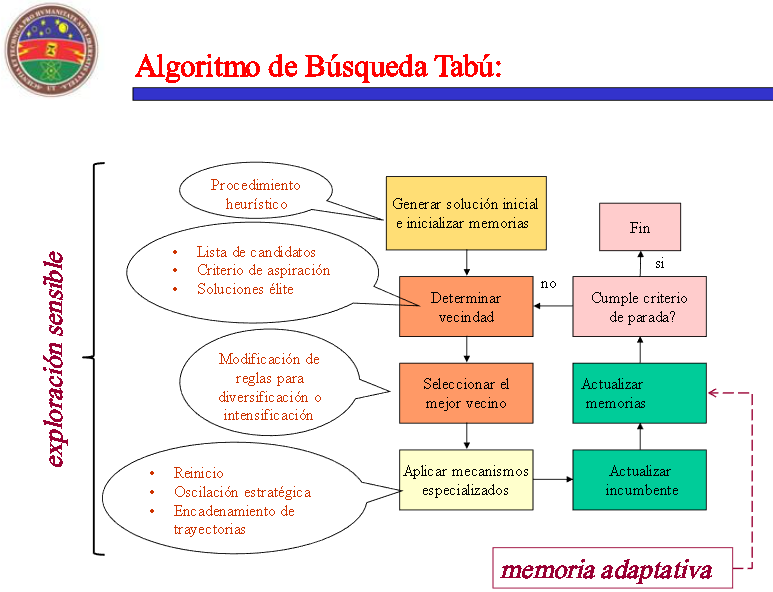
\includegraphics[width=8cm, height=5.5cm]{figuras/tabu.PNG}
\caption{Algoritmo de Búsqueda tabú - Tomado Universidad Tecnológica de Pereira, Colombia.}
\label{tabu} 
\end{center}
\end{figure}

A continuación, una investigación donde se evidencia la aplicación de este algoritmo:
\begin{enumerate}
\item En la investigación \textit{\textbf{“Búsqueda tabú para determinar
frecuencias en el transporte público”}}, \citep{martinez} se estudia el problema de determinación de frecuencias en el trasporte público utilizando un enfoque de optimización combinatoria. La determinación de frecuencias es llevada a cabo en las etapas de planificación estratégica y táctica de los sistemas de transporte público.

El \textbf{problema} consiste en determinar el intervalo de tiempo entre pasadas de buses subsecuentes de cada línea, considerando su ruta y la demanda de viajes. Las frecuencias impactan tanto a los usuarios como operadores. A los usuarios en el tiempo de espera. A los operadores en el costo de operación, dado que principalmente su costo está determinado por el tamaño de la flota requerida.

En este trabajo se consideraron dos formulaciones para el problema: objetivo único y multiobjetivo. La formulación de objetivo único \textbf{\textit{minimiza el tiempo total de viaje}} de los usuarios sujeto a una restricción en el tamaño de flota, mientras que la formulación multiobjetivo extiende la de objetivo único removiendo la restricción. Se proponen tres algoritmos, ver uno de ellos en la Figura ~\ref{tabu4}, para la resolución aproximada del problema basados en la metaheurística Búsqueda Tabú.

\begin{figure}[H]
\begin{center}
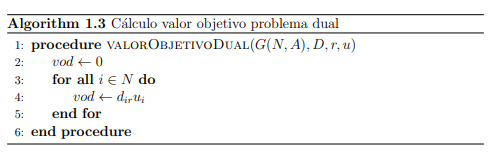
\includegraphics[width=6cm, height=2cm]{figuras/tabu4.PNG}
\caption{Función para el Cálculo valor objetivo problema dual.}
\label{tabu4} 
\end{center}
\end{figure}

Para la formulación de objetivo único los dos primeros algoritmos implementados producen una única solución, mientras que para la multiobjetivo el algoritmo produce un conjunto de soluciones no dominadas que representan diferentes compromisos entre los intereses de los usuarios y operadores. La propuesta es probada utilizando cuatro instancias reales del problema de diferentes dimensiones que \textbf{\textit{varían entre una decena y una centena de líneas de transporte}}. Se hace un estudio computacional exhaustivo para determinar el comportamiento de los algoritmos propuestos.

\begin{figure}[H]
\begin{center}
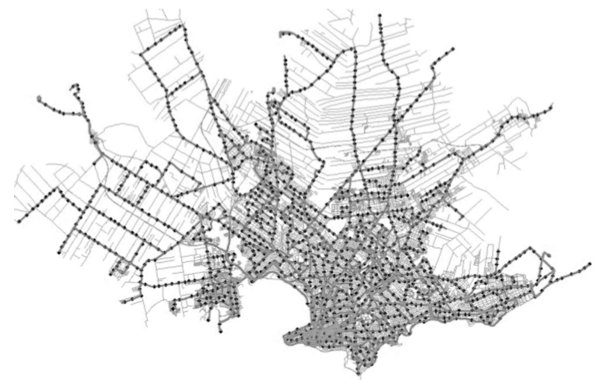
\includegraphics[width=6cm, height=3.5cm]{figuras/tabu2.PNG}
\caption{Red subyacente del caso Montevideo.}
\label{tabu2} 
\end{center}
\end{figure}

El caso de Montevideo, obsérvese la Figura ~\ref{tabu2}, es comparable en tamaño con los casos más grandes existentes en la literatura. Si bien para este problema no existen casos de estudios de referencia, los algoritmos implementados obtuvieron resultados en los rangos publicados en la literatura, entre 1\% y 5\%.

Los \textbf{resultados obtenidos} muestran que la metodología propuesta es capaz de mejorar las soluciones actuales en términos de tiempo de viaje y tamaño de flota, como se muestra en la Figura ~\ref{tabu3}. Además, para el caso de la variante multiobjetivo el método propuesto presenta diferentes soluciones alternativas con respecto al conflicto de intereses de los usuarios y operadores.

\begin{figure}[H]
\begin{center}
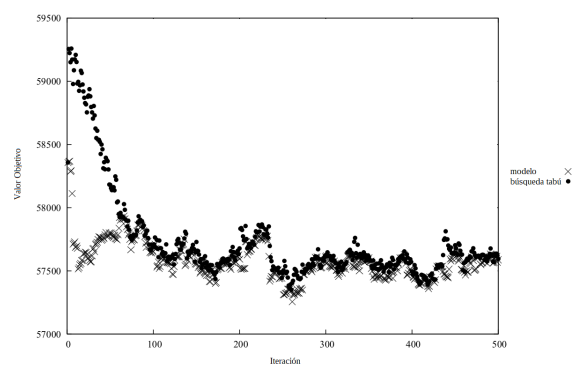
\includegraphics[width=6cm, height=3.5cm]{figuras/tabu3.PNG}
\caption{Evolución del valor objetivo en las 500 iteraciones A2 para el caso Montevideo.}
\label{tabu3} 
\end{center}
\end{figure}
\end{enumerate} 
%---------------------------------------------------------------------------
\subsection{\underline{\textbf{Temple o Recocido simulado (Simulated Annealing)}}}

El Simulated Annealing, como técnica de optimización combinatorial, se usa para afrontar problemas de gran complejidad matemática; cuenta con una estrategia de aceptación para las nuevas configuraciones que permite \textbf{salir de mínimos locales}, y encontrar soluciones de muy alta calidad, dentro de las cuales eventualmente puede estar el óptimo global \citep{anne}.

\begin{figure}[H]
\begin{center}
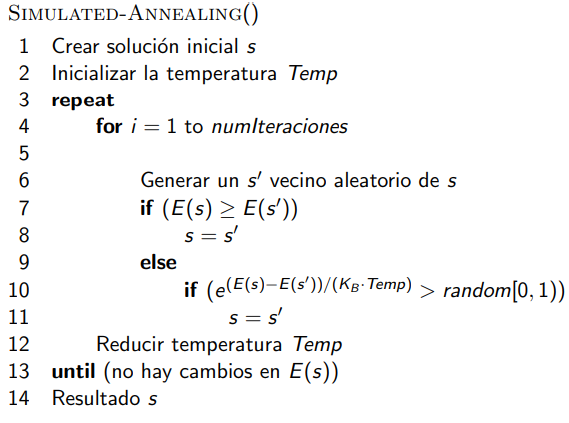
\includegraphics[width=6cm, height=4cm]{figuras/simu.PNG}
\caption{Algoritmo de Simulated Anneling - Tomado de Universidad de Zaragoza.}
\label{simu} 
\end{center}
\end{figure}

En algunos procesos metalúrgicos se calienta un material y después se enfría gradualmente de manera controlada, para aumentar el tamaño de los cristales que lo componen y reducir sus defectos.
Si la temperatura es suficientemente alta para asegurar un estado aleatorio y el enfriamiento es suficientemente lento para asegurar el equilibrio térmico los átomos alcanzarán un estado siguiendo un patrón que corresponde al mínimo de energía global para obtener un cristal perfecto\citep{simmu}.

Las características de este algoritmo son:
\begin{itemize}
    \item Se utiliza la analogía del recocido simulado para buscar soluciones de un problema de optimización cualquiera.
    \item Buscamos minimizar una cierta función de coste (la energía en el caso del recocido).
    \item Aun así (y en función de la temperatura) aceptaremos movernos a soluciones peores.
   \item De esa forma evitaremos enquistarnos en óptimos locales.
\end{itemize}
A continuación, una investigación donde se evidencia la aplicación de este algoritmo:
\begin{enumerate}
\item En la investigación \textit{\textbf{“Proceso de entrega del sistema de Enrutamiento utilizando Recocido Simulado”}}, \citep{sisw} el desarrollo del comercio electrónico y los sistemas de transporte inteligentes hace que las actividades logísticas sean una parte importante y cada vez mayor de la vida de las personas. La velocidad del transporte de carga hace que las empresas de logística sean más competitivas y los costos incurridos para la distribución son motivo de preocupación. Los mensajeros en una empresa de reparto son una de las principales fortalezas operativas, por lo que la determinación de la ruta debe estar bien definida.

\begin{figure}[H]
\begin{center}
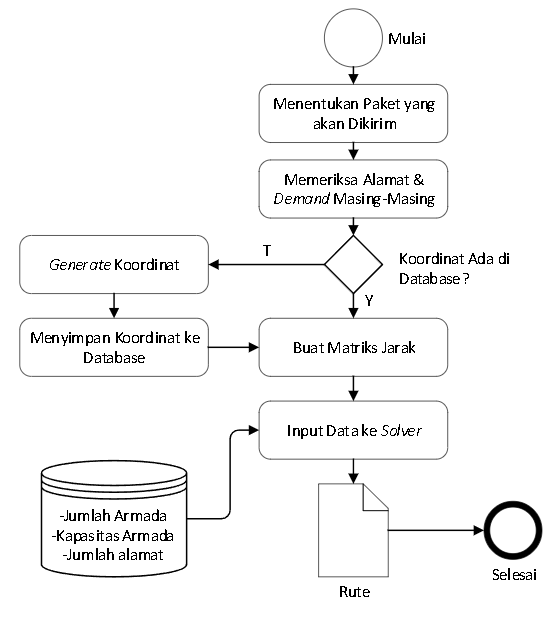
\includegraphics[width=6cm, height=5cm]{figuras/simu3.PNG}
\caption{Diagrama de Flujos del sistema de enrutamiento.}
\label{simu3} 
\end{center}
\end{figure}

Este estudio analiza la creación del sistema de enrutamiento y los procesos comerciales propuestos para la empresa de entrega (PT. X) mediante la aplicación del \textbf{problema} de enrutamiento de vehículos capacitados asimétricos (ACVRP) utilizando el algoritmo metaheurístico de \textit{recocido simulado} con una compensación entre la distancia total y la distancia máxima de una ruta 0.1; 0,5; y 0,9 , obsérvese el proceso en la Figura ~\ref{simu3}.

La finalización de ACVRP con Simulated Annealing comienza con la recopilación de datos relacionados con las teorías obtenidas. Estos datos incluyen datos de flota y horarios; PT. X Create Neighbor, actúa como una perturbación de la solución inicial para obtener una mejor solución que la solución anterior.

En que incluye los datos del cliente y el número de solicitudes; y procesos comerciales desde la programación hasta la entrega de los envíos. El siguiente paso después de recopilar los datos, el \textbf{procesamiento de datos} comienza con la obtención de datos de coordenadas geográficas del cliente obtenidos manualmente en Google Maps $(maps.google.com)$ con un total de 104 coordenadas (103 clientes y 1 depósito) que luego se hace una matriz de distancia entre coordenadas de clientes con unidades kilómetros, como se muestra en la Figura ~\ref{simu2}.

\begin{figure}[H]
\begin{center}
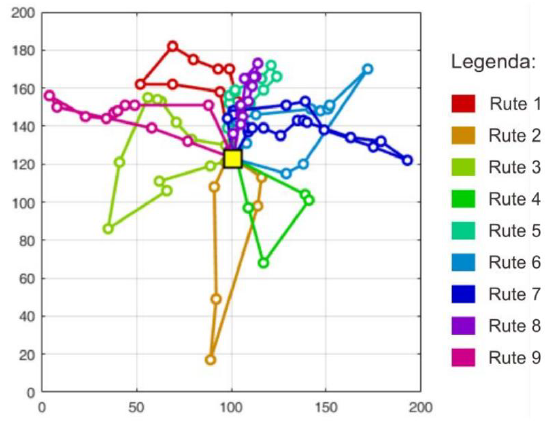
\includegraphics[width=6.5cm, height=4.5cm]{figuras/simu2.PNG}
\caption{Gráfico de red de rutas At = 0.1.}
\label{simu2} 
\end{center}
\end{figure}

La configuración en google maps no utiliza autopistas de peaje ya que los vehículos utilizados son motos. La \textit{descripción del problema} ACVRP a resolver con SA es el número de clientes (103 clientes), el número de vehículos (9 vehículos), la capacidad del vehículo (30 kg/moto), las solicitudes de los clientes y la matriz de distancia entre puntos.

El resultado obtenido fue que la \textit{\textbf{optimización del sistema}} de enrutamiento se ajusta a las necesidades del tomador de decisiones para enfocar su determinación de ruta, ya sea enfocada en la distancia total o en la distancia máxima de una ruta. El proceso comercial propuesto puede ahorrar hasta 2 horas.
\end{enumerate}

%---------------------------------------------------------------------------
\subsection{\underline{\textbf{Colonia de Hormigas}}}
El algoritmo de optimización Colonia de Hormigas, es un método metaheurístico introducido por Marco Dorigo a principios de 1990, el algoritmo está inspirado en el comportamiento natural de las hormigas en la búsqueda de sus alimentos. Dicha búsqueda consiste en explorar alrededor de la colonia de manera aleatoria (ya que las hormigas no cuentan con una buena visibilidad) para encontrar alguna fuente de alimento.\citep{dorigo} \par Una vez que han encontrado la fuente de alimento regresan al nido; durante ese regreso, las hormigas van depositando por el camino una sustancia llamada feromona (la feromona es una sustancia química que algunos animales segregan de ellos mismos y que cuya liberación puede llegar influenciar el comportamiento de los demás animales de la misma especie) y dicha feromona sirve para auxiliar al resto de las hormigas a seguir el mismo camino y encontrar la misma fuente de alimento. Cabe mencionar que el camino que las hormigas seguirán es el que mayor cantidad de feromonas tiene. \par
\textbf{Descripción del algoritmo}
    El algoritmo trabaja a partir de hormigas artificiales, que serán las encargadas de generar por cada iteración una solución factible al problema que se pretende resolver. Cada una construye su solución a partir de un grafo en donde cada nodo representa las posibles opciones que la hormiga podría elegir. La conexión que existe entre dos nodos, contiene información que las hormigas deben utilizar para poder elegir una de ellas, las cuales son \citep{dorigo}:
    \begin{itemize}
        \item \textbf{Información heurística:} representa la información a priori sobre la instancia del problema o información en tiempo de ejecución proporcionada por una fuente diferente de las hormigas.
        \item \textbf{Información de rastros de feromonas artificiales:} se mide la deseabilidad aprendida en el movimiento de un nodo a otro, lo cual busca imitar la feromona real que depositan las hormigas naturales. Esta información es modificada mientras que se ejecuta el algoritmo dependiendo de las soluciones encontradas por los insectos. 
    \end{itemize}
\begin{figure}[H]
 \begin{center}
       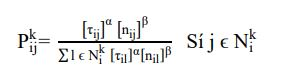
\includegraphics[width=7cm, height=2cm]{figuras/hormigas1.JPG}
      \caption{Probabilidad de elegir un nodo.}
      \label{f4hormiga} 
      \end{center}
\end{figure}

\begin{figure}[H]
 \begin{center}
       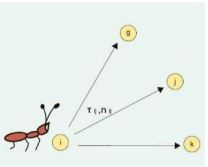
\includegraphics[width=7cm, height=4cm]{figuras/hormigas.JPG}
      \caption{Una hormiga estando en el nodo i, a punto de elegir un nodo para visitar.}
      \label{f5hormiga} 
      \end{center}
\end{figure}

\par A continuación, una investigación respecto a este algoritmo de Colonia de Hormigas:
\begin{enumerate}
\item En la tesis \textbf{\textit{“Segmentación de imágenes médicas mediante algoritmos de Colonia de Hormigas”}} Maestría en Informática. Pontifica Universidad Católica del Perú. Lima-Perú, \citep{calderon} se planteó  un procedimiento de segmentación de imágenes médicas basado en la metaheurística de Algoritmos de Colonia de Hormigas. Fue implementado mediante hormigas artificiales con el objeto de realizar tareas específicas de procesamiento de imágenes. Este procedimiento fue aplicado a imágenes de Resonancias Magnéticas Cerebrales - buscando la extracción de los segmentos correspondientes a la Materia Gris, Materia Blanca y Líquido Cefalorraquídeo- y la segmentación obtenida fue de una calidad superior a la de los algoritmos actualmente existentes para esta tarea. (Ver Figura ~\ref{f3hormiga})
\begin{figure}[H]
 \begin{center}
       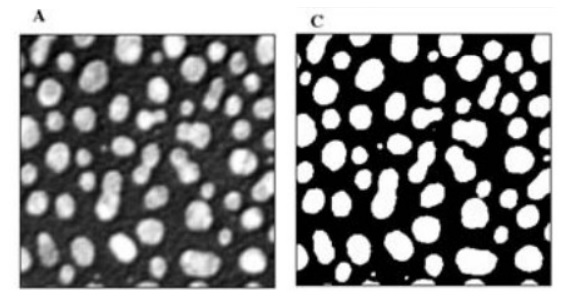
\includegraphics[width=7cm, height=3cm]{figuras/hormigas3.JPG}
      \caption{Imagen original e imagen segmentada}
      \label{f3hormiga} 
      \end{center}
\end{figure}
\textbf{Problema de la investigación}
    Por ejemplo la rinitis atrófica, antes de realizar el cálculo de áreas es necesario depurar las imágenes obtenidas para remover imperfecciones y hacer el cálculo de áreas más preciso. Esta labor de pre-procesamiento en caso de ser realizada manualmente demanda considerable tiempo y esfuerzo, lo que por el contrario puede ser realizado de manera rápida y eficiente por una computadora y un buen algoritmo. Este es uno de los aspectos donde el uso de computadores resulta beneficioso para el análisis de imágenes.\par 
 \textbf{Resultados obtenidos}
    Son dos las principales métricas que el experimento buscó obtener. La primera es el tiempo de segmentación, que es medido por el Software construido desde el inicio del proceso hasta que los segmentos son producidos. Para la configuración descrita, se obtuvo un tiempo de segmentación de aproximadamente 300 segundos.\par    
    La segunda métrica a obtener es la calidad de la segmentación producida. Para evaluar el desempeño del algoritmo compararemos los segmentos producidos por el algoritmo contra los segmentos de referencia contenidos en la base de datos, como lo muestra la Figura~\ref{f2hormiga}.
\begin{figure}[H]
 \begin{center}
       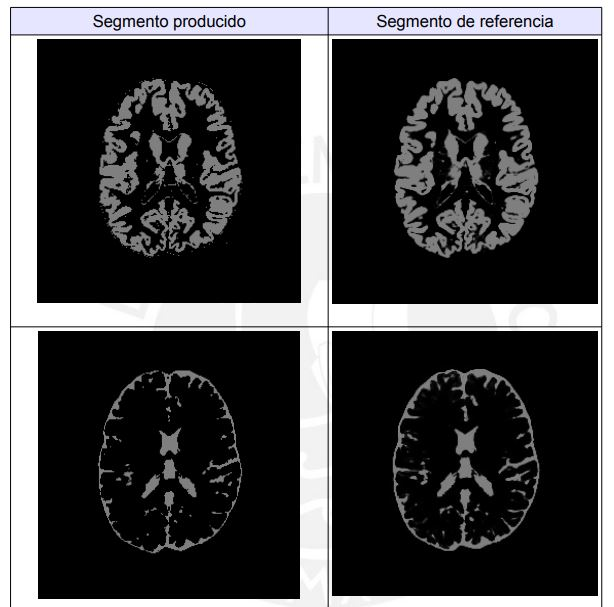
\includegraphics[width=7cm, height=5cm]{figuras/hormigas2.JPG}
      \caption{Segmentos producidos versus. Segmentos de referencia}
      \label{f2hormiga} 
      \end{center}
\end{figure}
Finalmente, los resultado experimentales muestran similitudes altas para ciertos segmentos -en valores de JSI de 0.93- mientras para otros la calidad de la segmentación si bien es inferior se mantiene en niveles aceptables. Asimismo, incluso en los mejores segmentos el porcentaje de falsos negativos es alto lo que implica que varios píxeles esta siendo omitidos durante el proceso de segmentación. La calidad de los segmentos obtenidos es buena y es comparable con los algoritmos principales que sobre el mismo set de datos llegan a valores de JSI de 0.9.
\end{enumerate}

%---------------------------------------------------------------------------
\subsection{\underline{\textbf{Enjambre de partículas}}}
El algoritmo de optimización por enjambre de partículas (PSO), fue originalmente desarrollado por James Kennedy y Russell Eberhart en 1995, es un algoritmo del área de la inteligencia artificial de la rama de inteligencia de enjambres. Está inspirada en el comportamiento social de los seres vivos \citep{kennedy}. \par
El algoritmo de optimización por enjambre de partículas se inspira en la evolución en el comportamiento colectivo, principalmente trata de imitar el comportamiento social de varios grupos de animales como lo son los cardúmenes, parvadas, manadas, etc. \citep{kennedy1995}. El algoritmo se basa en población de individuos, ha demostrado ser eficiente para la solución de problemas complejos.\par

En términos generales, la estructura de un algoritmo PSO para optimizar (maximizar o minimizar) una función con una o múltiples variables sigue los siguientes pasos\citep{Optimiza}:
\begin{enumerate}
    \item Crear un enjambre inicial de n partículas aleatorias. Cada partícula consta de 4 elementos: una posición que representa una determinada combinación de valores de las variables, el valor de la función objetivo en la posición donde se encuentra la partícula, una velocidad que indica cómo y hacia donde se desplaza la partícula, y un registro de la mejor posición en la que ha estado la partícula hasta el momento.
    \item Evaluar cada partícula con la función objetivo.
    \item Actualizar la posición y velocidad de cada partícula. Esta es la parte que proporciona al algoritmo la capacidad de optimización. En el apartado Mover partícula se describe con detalle el proceso.
    \item Si no se cumple un criterio de parada, volver al paso 2.
    
    \begin{figure}[H]
    \begin{center}
       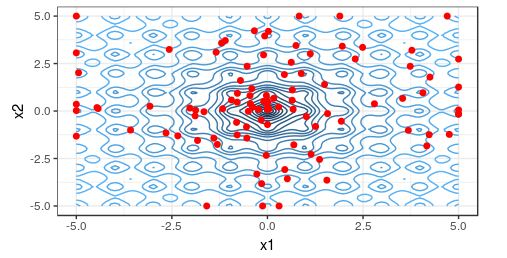
\includegraphics[width=7cm, height=4cm]{figuras/enjambre2.JPG}
      \caption{Animación de cómo avanza la búsqueda del mínimo.1}
      \label{f1enjambre} 
      \end{center}
    \end{figure} 

    \begin{figure}[H]
    \begin{center}
       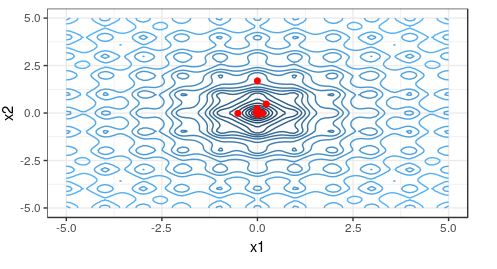
\includegraphics[width=7cm, height=4cm]{figuras/enjambre1.JPG}
      \caption{Animación de cómo avanza la búsqueda del mínimo.2}
      \label{f2enjambre} 
      \end{center}
    \end{figure} 
    
\end{enumerate}
\par A continuación, una investigación respecto a este algoritmo de Enjambre de partículas:
\begin{enumerate}
    \item En la tesis \textbf{\textit{“Reconfiguración del Sistema Eléctrico de la Ciudad de Puno usando la Técnica de Optimización Binaria por Enjambre de Partículas para Reducir la Sobrecarga de la S.E. Bellavista”}} Ingeniería Eléctrica. Universidad San Agustín de Arequipa. Arequipa-Perú, \citep{cornejo} se propuso una solución al problema de sobrecarga en la subestación Bellavista, perteneciente a la concesionaria de distribución eléctrica Electro Puno S.A.A, subestación que alimenta de energía eléctrica a la Ciudad de Puno utilizando la técnica de optimización binaria por enjambre de partículas. \par
    La fuente de información que se utilizó para el desarrollo del trabajo fue la base de datos de la concesionaria Electro Puno S.A.A. con la cual se modeló el sistema eléctrico en el software de sistemas de potencia Digsilent y posteriormente se realizó la reconfiguración del sistema eléctrico con el software de cálculo numérico Matlab y el paquete de funciones de sistemas de potencia Matpower.

    \textbf{Problema de la investigación} Actualmente el sistema eléctrico de la ciudad de Puno presenta sobrecargas en la subestación Bellavista en uno de sus 2 transformadores, en horas de alta demanda (desde las 18:00 a 24:00 horas), según los informes técnicos de Osinergmin. Estos hechos están ocasionando deterioro del tiempo de vida de conductores, deterioro del tiempo de vida del transformador de la subestación, elevadas caídas de tensión y aumento en la probabilidad de fallas por sobrecarga. Adicionalmente en estas condiciones las pérdidas del sistema son bastante mayores que las que se darían en condiciones normales.\par
    \textbf{Resultados obtenidos}
    La reconfiguración permitió la eliminación de la sobrecarga del transformador T101 en la subestación Bellavista como se muestra en la tabla 5.11, donde se ve que la potencia antes de la reconfiguración era de 5.72 MVA para una cargabilidad del 105.2\% y después de la reconfiguración la potencia es de 4.92 MVA para una cargabilidad de 91.08\%.(Ver Figura ~\ref{f3enjambre})

    \begin{figure}[H]
    \begin{center}
       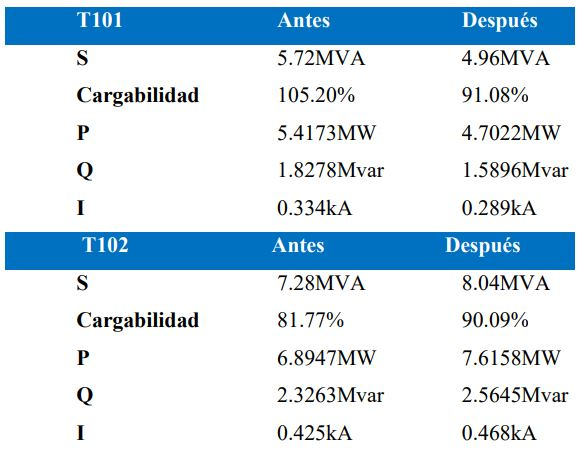
\includegraphics[width=7cm, height=5cm]{figuras/enjambres3.JPG}
      \caption{Comparación de resultados de la cargabilidad de los transformadores}
      \label{f3enjambre} 
      \end{center}
    \end{figure}    
    
\end{enumerate}

%---------------------------------------------------------------------------
\section{\textbf{Conclusiones}}
Este informe presentó información relevante acerca de cuatro Algoritmos Metaheurísticos empleados en la Inteligencia Artificial, explicándose también los conceptos teóricos relacionados a ellos. Además de permitir conocer sobre algunas investigaciones que se vienen realizando año a año, entendiendo las diversas aplicaciones de las ciencias de la computación en la vida diaria. Concluimos que la mayoría analiza la problemática y dependiendo de sus características se establecieron los procesos así como las técnicas a emplear, para usar las Metaheurísticas, siendo este un campo tan importante donde se evidencia el intento de alcanzar una mayor eficiencia y efectividad en la exploración del espacio de búsqueda. Finalmente, las investigaciones en la informática expuestas en este trabajo de recopilación, sirven como antecedentes y base a futuros investigadores a nivel nacional e internacional, que pueden ser usados tanto en el área comercial o académico
%-------------------------------------------------------
\medskip
\bibliography{refer}
\end{document}